\documentclass[UTF8]{ctexart}

\usepackage{subfiles}  

%下面的语句, 引入你的头部设置文件
\usepackage{C:/phpStorm_proj/02_myself_ID_EGO/+100_latex_all_math_sel/myPreamble} 
%必须是绝对路径,才能让各个tex在单独编译时使用到

\title{积分}


%---------------------------------


\begin{document}
	\tableofcontents % 生成目录
	\date{} % 若不写这句, 则默认也会渲染出日期, 所以我们要手动赋空值
	\maketitle  %这行代码, 让你前面的 title, author, date生效
	
	\part{定积分 definite integral}
	
	
	\section{``定积分"的定义}
	
	1. 曲线函数f(x), 在x轴上有界, 比如端点是[a,b].
	
	2. 然后, 我们在[a,b]这段区间上, 任意插入n个分点, 分成n个小区间. 它们不要求等分. 每个小区间的长度就是 $ \Delta x_1, \Delta x_2,..., \Delta x_n$.
	
	3. 在每个Δ小区间上, 任取一点 $ \xi_i$. 这点的函数值(即y轴上的高度), 就是 $ y=f(\xi_i)$.
	
	4. 这样, 我们就能得到每一个Δ小区间, 所在的``长方形细条的面积"了, 即 $= \text{宽} \Delta x_i \cdot \text{高}f(\xi_i)$
	
	5. 把所有这些Δ小区间的``长方形细条面积", 全加起来, 就是该曲线到x轴间的面积的近似值. $ = \sum_{i=1}^n \Delta x_i\cdot f(\xi _i) $
	
	6. 我们令其中 x轴宽度最大的那个Δx小区间 (假设起名为λ, 即$ \lambda =\max \left\{ \varDelta x_1,...,\varDelta x_n \right\} $), 我们让这个λ, 极限趋向于0. 这样, 既然最大的 Δx小区间 都趋近于0了, 其他比它更小的 Δx小区间, 就都统统被约束, 也都趋向于0了. 这样, 它们的``长方形细条的面积之和", 就能精确的等于``函数曲线到x轴之间的面积"了, 而不仅仅是``近似"了. \\
	
	即: 
	$	\lim_{x\rightarrow 0}\sum_{i=1}^n{\underset{\text{高}}{\underbrace{f\left( \xi _i \right) }}\cdot \underset{\text{宽}}{\underbrace{\varDelta x_i}}=\underset{\text{定积分}}{\underbrace{\int_a^b{f\left( x \right)}dx}}}	$ \\
	
	各部分的名字是:
	$
	\int_{\text{下限}a}^{\text{上限}b}{\underset{\text{被积表达式}}{\underbrace{\underset{\text{被积函数}}{\underbrace{f\left( x \right) }}\ d\underset{\text{积分变量}}{\underbrace{\left( x \right) }}}}}
	$
	
	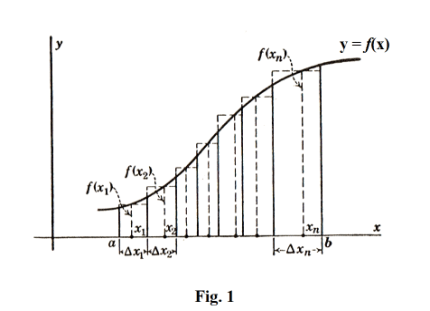
\includegraphics[width=0.5\textwidth]{/0060.png}
	
	
	
	
	
	\section{定积分的性质}
	
	\subsection{若 b=a, 则 $ \int_a^a f(x) = 0$}
	
	\subsection{$ \int_a^b f(x) = -  \int_b^a f(x)$  ← 交换上下限, 定积分的值要变号}
	
	\subsection{$\int_a^b (\alpha \cdot f(x) + \beta \cdot g(x)) dx = \alpha \int_a^b  f(x) dx + \beta \int_a^b  g(x) dx$ ← 即, 积分可以拆开, 常数可以提到外面去}
	
	\subsection{ 若 $ a < c < b$, 则 $ \int_a^b f(x) dx = \int_a^c f(x) dx + \int_c^b f(x) dx $ ← 其实就是原先的一步走, 分成两步走而已.}
	
	
	\subsection{ 若 $ a < b < c$, 则: $ \int_a^b f(x) dx = \int_a^c f(x) dx - \int_c^b f(x) dx$}
	
	
	
	
	
	
	
	
	
	
	
	
	
	
	
	
\end{document}


